% Appendix: detailed analyses of the direct and CausalCoT runs.
% Moved out of the main text on 2026-09-27 to keep Sects. 4-5 short.
% Include it by setting \includeappendixtrue in main.tex.
% Note: written before the question-only prior run; the TODOs on the
% prior probe (Sect. "What the current design can and cannot detect")
% are answered in the main text, Sect. 5.3.

\section{Detailed analysis plan}
\label{app:analysis}

This study is exploratory. It was designed to test the feasibility of the experiments planned for the first author's thesis, and we use its results mainly to establish what the current design can and cannot show. We distinguish three kinds of analysis and report them separately.

\emph{Pre-stated tests.} For H1, the gap between commonsensical and anti-commonsensical accuracy is computed on matched pairs, with a percentile bootstrap interval (10,000 resamples) and an exact McNemar test; the gap to nonsensical items uses Newcombe's interval for independent proportions. For H1b, we compute the paired difference in mean $P(\text{Yes})$ between commonsensical and anti-commonsensical items on the query types that ask whether $X$ affects $Y$ (conditional probability, average treatment effect and its version on the treated, natural direct and indirect effects, and counterfactuals), separately for items whose correct answer is Yes and No. For H2, accuracy is compared across rungs \todo{test: $\chi^2$ or logistic regression of correctness on rung}. Direct and CausalCoT accuracy are compared on the same items with McNemar's test. Accuracy is reported with 95\% Wilson intervals. Intervals are not corrected for multiplicity: H1b alone involves sixteen intervals (four models, two answers, two conditions), so an isolated interval that barely excludes zero should be read with caution.

\emph{Descriptive measures.} Thresholding $P(\text{Yes})$ at 0.5 mixes two things: whether the model's preference follows the correct answer, and where its overall bias lies. We therefore also report the \emph{Yes rate}, the share of items answered ``Yes''; \emph{discrimination}, the area under the ROC curve (AUROC) of $P(\text{Yes})$ against the correct answer, pooled and averaged within query types \todo{stratified AUROC with bootstrap CI}, where 0.5 means that the probability carries no information about the answer; and \emph{name sensitivity}, the share of matched pairs whose thresholded answer flips when the variable is renamed. To read null results we treat differences within $\pm 0.04$ as negligible. This bound was fixed after the direct runs, from the 1.8-point gap Jin et al.\ report for GPT-4 \cite{jin2023cladder}, and is used descriptively rather than as a formal equivalence test.

\emph{Post hoc diagnostics.} After the direct results we added four checks of the design itself, reported in Sect.~\ref{sec:res-limits}. (i) \emph{Belief congruence.} If anti-commonsensical names lower $P(\text{Yes})$, they penalize items whose correct answer is Yes but help items whose correct answer is No, so the pooled H1 gap can be close to zero even when the effect is present. We split relational pairs into belief-congruent items (commonsensical with answer Yes, anti-commonsensical with answer No) and belief-incongruent items (the reverse) and compare their accuracy, as in studies of content effects on reasoning in humans and LLMs \cite{dasgupta2024language}. (ii) \emph{Prior probe.} The account assumes that the models hold the commonsense prior that the names should trigger. We test this by presenting the question of each matched pair alone, without the background or the given information, and reading $P(\text{Yes})$ as in Sect.~\ref{sec:prompting}; the commonsensical minus anti-commonsensical difference in this \emph{prior} $P(\text{Yes})$ measures how much prior there is to override. (iii) \emph{Question polarity.} CLadder asks some relational questions about an increase and others about a decrease; a commonsense prior favours ``Yes'' only for the former. We code each question's polarity and recompute H1b on increase questions. (iv) \emph{Noise floor.} For the two quantized models, $P(\text{Yes})$ depends slightly on batching. We re-score 200 items one at a time and report the answer-flip rate, which bounds how much of the name sensitivity could be numerical noise.

% EDITOR: toy example of a "failure DAG" and "model's error surface" -> the co-occurrence graph was dropped; the query-type x topology heatmap replaces it.

\section{Detailed results of the direct and CausalCoT runs}
\label{app:results}

We first describe how the models answer (Sect.~\ref{sec:res-behaviour}), because answer bias and weak discrimination constrain every later comparison. We then report the pre-stated tests (Sects.~\ref{sec:res-names} and~\ref{sec:res-where}), the exploratory CausalCoT condition (Sect.~\ref{sec:res-cot}), and the post hoc diagnostics that show what the current design can and cannot detect (Sect.~\ref{sec:res-limits}). SmolLM2 answers ``No'' to all but 0.1\% of the items, so its accuracy equals the share of ``No'' answers in each subset; we report it, but draw no inferences from it.

\subsection{The models answer close to chance and with strong bias}
\label{sec:res-behaviour}

All four models are between 0.50 and 0.60 accurate on every variant (Table~\ref{tab:variants}, Fig.~\ref{fig:acc-variant}), on a set in which half of the correct answers are ``Yes''. Their Yes rates differ widely: 0.1\% for SmolLM2, 33\% for Phi-3.5, 48\% for Qwen2.5-7B, and 50\% for Qwen2.5-1.5B. Discrimination is weak (Fig.~\ref{fig:discrimination}). On all 3,000 direct items the pooled AUROC is 0.50 for SmolLM2, 0.53 for Qwen2.5-1.5B, 0.61 for Phi-3.5, and 0.62 for Qwen2.5-7B \todo{stratified AUROC}. For the two small models the $P(\text{Yes})$ distributions of Yes and No items almost coincide; for the two larger ones they differ, but largely through a mass of confident ``No'' answers present for both kinds of item. The effect of the names is therefore measured on models that use the given structure only weakly, which limits how large a name effect could be and how it can be interpreted (Sect.~\ref{sec:res-limits}).





\begin{figure}[!htbp]
  \centering
  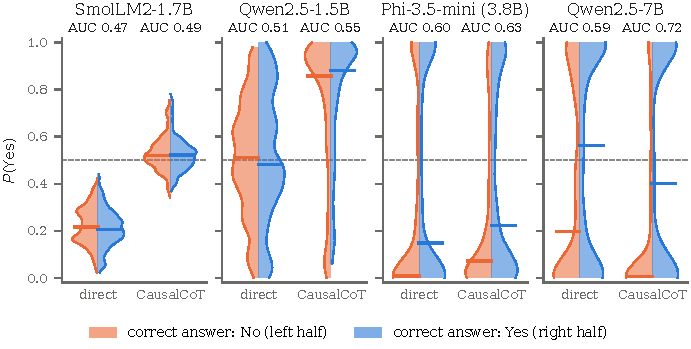
\includegraphics[width=\textwidth]{./figures/discrimination_pyes.pdf}
  \caption{Distribution of $P(\text{Yes})$ for items whose correct answer is No (left halves) and Yes (right halves), on the same 450 items in the direct and CausalCoT conditions; horizontal ticks are medians. AUROC $=0.5$ means that $P(\text{Yes})$ carries no information about the correct answer.}
  \label{fig:discrimination}
\end{figure}

\subsection{Pre-stated tests of word plausibility (H1, H1b)}
\label{sec:res-names}

\paragraph{H1.} On the 1,000 matched pairs, no model is significantly less accurate on anti-commonsensical items (Fig.~\ref{fig:forest}a). The gaps are $+0.002$ (SmolLM2), $+0.014$ (Qwen2.5-1.5B, 95\% CI $-0.013$ to $0.042$), $+0.014$ (Phi-3.5, $-0.014$ to $0.042$), and $-0.025$ (Qwen2.5-7B, $-0.055$ to $0.005$), with no McNemar test below $p = 0.12$. Every upper bound lies at or below $0.042$. Commonsensical and nonsensical accuracy do not differ either (largest gap $+0.034$, Phi-3.5, 95\% CI $-0.009$ to $0.077$). As Sect.~\ref{sec:res-limits} shows, however, this pooled gap is not a sensitive test of the account.

\paragraph{H1b.} The shifts in $P(\text{Yes})$ differ between models (Fig.~\ref{fig:forest}b). Phi-3.5 shifts in the predicted direction on both kinds of item, assigning about 0.05 less probability to ``Yes'' on anti-commonsensical items (Yes items: 95\% CI $0.004$ to $0.103$; No items: $0.001$ to $0.098$). Both Qwen models shift in the opposite direction on Yes items ($-0.044$ and $-0.050$, both intervals excluding zero), and SmolLM2's shifts are below 0.01. The result is therefore heterogeneous rather than null: one model shows a small effect in the predicted direction and two show small effects in the opposite direction. All of these intervals lie close to zero and are uncorrected \todo{Holm-adjusted intervals}, and none of the shifts exceeds 0.06.

\paragraph{Name sensitivity.} The names change individual answers. Renaming one variable flips the answer on 20\% (Qwen2.5-1.5B), 21\% (Phi-3.5), and 24\% (Qwen2.5-7B) of pairs, and the paired probabilities are only moderately correlated (Spearman $\rho = 0.65$--$0.76$; Fig.~\ref{fig:scatter}). The flips are close to symmetric: in Qwen2.5-7B, 107 pairs are correct only under the commonsensical name and 132 only under the anti-commonsensical one, and for every model the share of pairs below the diagonal is between 0.45 and 0.56. Whether these flips reflect the names or numerical noise cannot be decided without a noise floor (Sect.~\ref{sec:res-limits}).

\begin{figure}[!htbp]
  \centering
  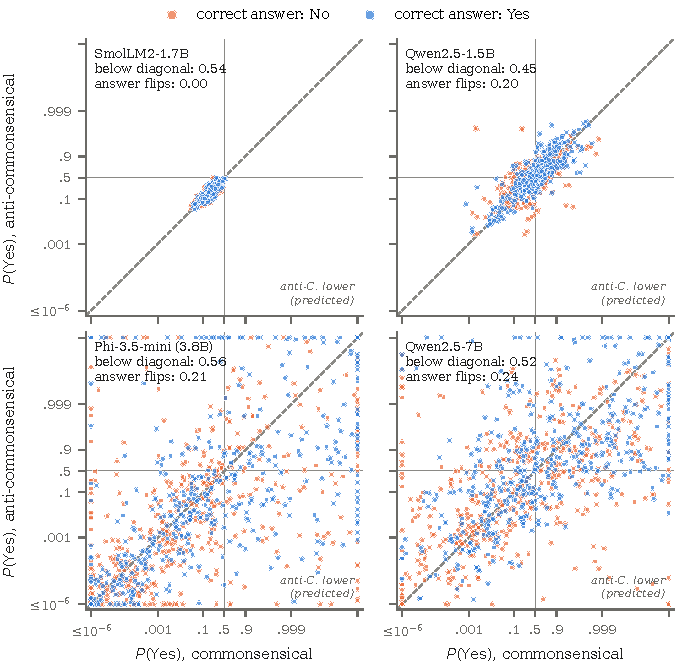
\includegraphics[width=0.78\textwidth]{./figures/paired_pyes_scatter.pdf}
  \caption{$P(\text{Yes})$ for the 1,000 matched pairs in the direct condition: the commonsensical item on the $x$-axis and its anti-commonsensical twin, with the same graph, probabilities, and answer, on the $y$-axis (logit scale; values beyond $10^{-6}$ are drawn at the edge). The plausibility account predicts points below the diagonal for relational questions about an increase; the panel pools all query types and both question polarities. Colours mark the correct answer. \emph{Answer flips}: share of pairs whose thresholded answer differs between the two names.}
  \label{fig:scatter}
\end{figure}

\begin{figure}[!htbp]
  \centering
  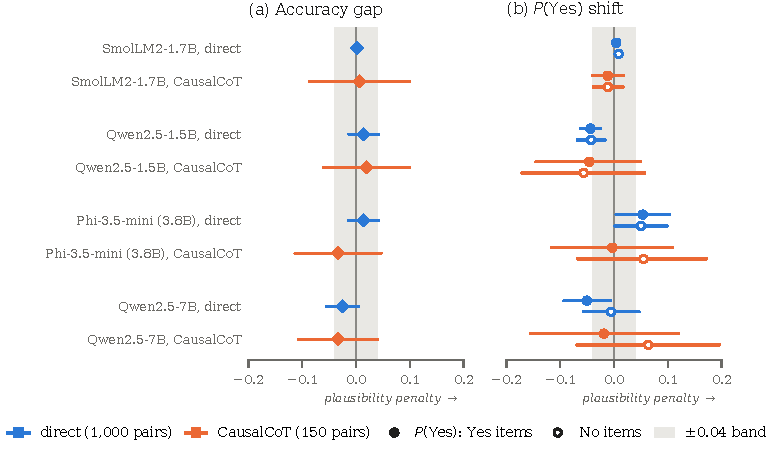
\includegraphics[width=\textwidth]{./figures/forest_effects.pdf}
  \caption{Commonsensical minus anti-commonsensical effects with 95\% bootstrap intervals (uncorrected), direct (1,000 pairs) and CausalCoT (150 pairs). Positive values are the predicted plausibility penalty. (a) Accuracy gap (H1). (b) Shift in mean $P(\text{Yes})$ on relational items (H1b), separately for items whose correct answer is Yes (filled) and No (open). The shaded band marks $\pm 0.04$.}
  \label{fig:forest}
\end{figure}

\subsection{Accuracy varies with the query type more than with the rung (H2)}
\label{sec:res-where}

Accuracy does not decrease with the rung. For every model whose accuracy varies, L1 is the lowest rung; for Qwen2.5-7B it is 0.52, 0.64, and 0.57 at L1--L3 \todo{95\% CIs and test}. The larger differences are between query types within a rung (Fig.~\ref{fig:heatmap}). Pooled over the three informative models, the average treatment effect is above chance in most topologies (0.62--0.80, except the instrumental-variable and diamondcut graphs, 0.49 and 0.55), and the natural direct and indirect effects at L3 are at or above chance in every topology where CLadder generates them (0.52--0.71). The choice of adjustment set and collider bias, both at L2, are at or below chance, and collision graphs, which contain only marginal, explaining-away, adjustment-set, and collider-bias questions, are the hardest topology (0.34--0.47).

The low cells reflect constant answers rather than difficult numbers. Phi-3.5 and Qwen2.5-7B answer ``No'' to every collider-bias question, Qwen2.5-7B answers ``No'' to 99\% of adjustment-set questions, and Phi-3.5 answers ``No'' to 99\% of marginal-probability questions, although the correct answer is ``Yes'' on 47--54\% of the items of each of these query types. In these cells the answer follows the wording of the question template, not the graph or the probabilities it states. Because each rung contains different query types, rung-level accuracy largely reflects which query types receive a constant answer and how often that answer is correct; a comparison of rungs therefore requires balanced accuracy within query types \todo{balanced accuracy by rung}.

\begin{figure}[!htbp]
  \centering
  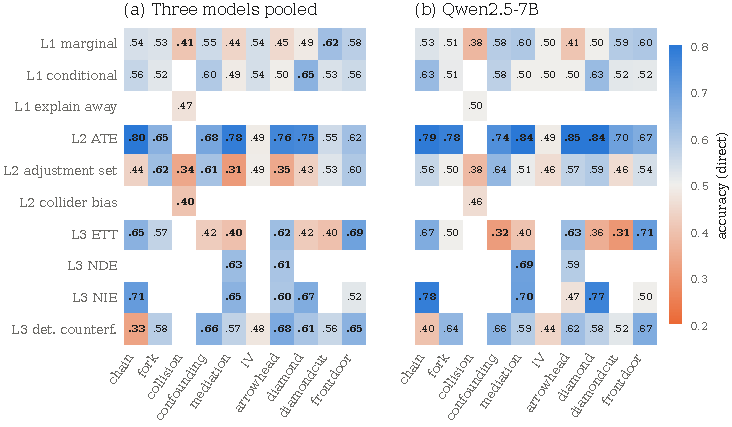
\includegraphics[width=\textwidth]{./figures/heatmap_query_topology.pdf}
  \caption{Direct-condition accuracy by query type (rows, grouped by rung) and graph topology (columns). (a) Pooled over Qwen2.5-1.5B, Phi-3.5, and Qwen2.5-7B; (b) Qwen2.5-7B alone. SmolLM2 is omitted because its accuracy in each cell equals the share of ``No'' answers. Bold values have a 95\% Wilson interval that excludes 0.5; blank cells are combinations that CLadder does not generate.}
  \label{fig:heatmap}
\end{figure}

\subsection{Reasoning first shifts the bias more than the accuracy (exploratory)}
\label{sec:res-cot}

Table~\ref{tab:cot} and Fig.~\ref{fig:acc-cot} compare the two conditions on the same items. Reasoning first raises accuracy significantly only for Qwen2.5-7B, from 0.57 to 0.64 (paired difference $+0.073$, 95\% CI $0.029$ to $0.118$, McNemar $p = 0.002$), which is also the only model whose discrimination clearly improves (AUROC 0.59 to 0.72 on these items; Fig.~\ref{fig:discrimination}). Its subset was enlarged after the first CausalCoT results \todo{final $N$ for Qwen2.5-7B, and the result on the original 150 pairs}. The changes for Qwen2.5-1.5B ($+0.047$, $p = 0.16$), Phi-3.5 ($+0.022$, $p = 0.43$), and SmolLM2 ($-0.007$) are not significant, and their AUROC stays between 0.47 and 0.55. For the two small models, reasoning mainly moves the threshold. Qwen2.5-1.5B answers ``Yes'' to 78\% of items instead of 50\%. SmolLM2 moves from confident ``No'' answers to probabilities clustered near 0.52, so its 63\% ``Yes'' rate reflects answers close to indifference rather than a preference for ``Yes''. No paired accuracy gap and no $P(\text{Yes})$ shift differs from zero after reasoning (Fig.~\ref{fig:forest}, orange), but with 150 pairs these intervals are about $\pm 0.08$ wide. After regeneration at 1,024 tokens, 3--8\% of traces per model still reached the limit, at similar rates across variants.

\begin{table}[!htbp]
\centering
\caption{Direct and CausalCoT conditions on the same 450 items per model (150 pairs + 150 nonsensical items): accuracy, commonsensical minus anti-commonsensical accuracy on matched pairs (95\% bootstrap CI), and share of CausalCoT traces that reached the 1,024-token limit. SmolLM2's direct gap is undefined because it answers ``No'' to every item.}
\label{tab:cot}
\scriptsize
\begin{tabular}{lccccc}
\toprule
Model & Acc.\ direct & Acc.\ CoT & Gap direct & Gap CoT & Trunc. \\
\midrule
\csname @@input\endcsname tables/cot_rows.tex
\bottomrule
\end{tabular}
\end{table}

The traces suggest why reasoning helps so little. Deterministic counterfactual questions provide no probabilities, only logical relations, yet 81\% of Qwen2.5-1.5B traces and 74\% of SmolLM2 traces on these items state probability values, against 12\% for Phi-3.5 and 9\% for Qwen2.5-7B (43 items per model, flagged by a text heuristic that detects numeric probability statements). Other traces misidentify the query type, for example by treating a choice between two adjustment strategies as an average treatment effect and then waiting for probabilities that the question does not contain. On this small sample, the model that invents data least is also the only one that benefits from reasoning.

\subsection{What the current design can and cannot detect}
\label{sec:res-limits}

The null result on H1 and the mixed result on H1b do not, on their own, count against the plausibility account, because the design has limits that bear directly on these tests. Table~\ref{tab:limits} summarizes them together with the diagnostics of Appendix~\ref{app:analysis} and the changes planned for the thesis experiments.

\emph{The pooled accuracy gap is insensitive to the effect.} If anti-commonsensical names lower $P(\text{Yes})$, the resulting loss on Yes items and gain on No items cancel in the pooled gap, since CLadder is balanced between the two answers. The belief-congruence split separates them: \todo{accuracy on congruent vs.\ incongruent pairs, per model, with CI}.

\emph{The prior is assumed, not measured.} A null result on H1b could mean that the given structure overrides the names, or that models of this size hold no prior for the names to express. The prior probe separates these readings: \todo{commonsensical minus anti-commonsensical prior $P(\text{Yes})$ per model}. \todo{If the prior gap is large: the in-context null means the names do not carry the prior into the answer. If it is small: the test cannot distinguish the two readings at this scale.}

\emph{The predicted shift depends on the question's polarity.} A commonsense prior should lower $P(\text{Yes})$ on anti-commonsensical items for questions about an increase, but not for questions about a decrease, and H1b pools both. \todo{H1b on increase questions only}.

\emph{Name sensitivity has no noise floor.} The 20--24\% of answer flips cannot be attributed to the names until they are compared with the flips produced by numerical noise alone: \todo{flip rate at batch size 1 vs.\ batched, for Phi-3.5 and Qwen2.5-7B}.

Two further limits concern the comparison groups. Nonsensical items use their own parameters and are compared as a group, not as pairs, so differences between them and commonsensical items mix the names with the numbers. And because the models answer near chance and with strong bias (Sect.~\ref{sec:res-behaviour}), accuracy leaves little room for any name effect to appear; $P(\text{Yes})$ and AUROC are the more informative measures in this regime.

\begin{table}[!htbp]
\centering
\caption{Limitations of the current design, what they imply for the results reported here, and how the thesis experiments address them.}
\label{tab:limits}
\scriptsize
\renewcommand{\arraystretch}{1.15}
\begin{tabular}{p{0.27\textwidth}p{0.33\textwidth}p{0.32\textwidth}}
\toprule
Limitation & Consequence here & Planned change \\
\midrule
Pooled accuracy gap (H1) & Effect on Yes and No items cancels; a null is expected even if the account holds & Belief-congruence split as the primary accuracy test \\
No measure of the prior & A null on H1b cannot separate ``structure overrides names'' from ``no prior'' & Prior probe on every matched pair \\
Mixed question polarity & Predicted shifts may cancel within H1b & Code polarity; test increase and decrease questions separately \\
No noise floor & 20--24\% name flips cannot be attributed to the names & Batch-size-1 re-scoring; unquantized inference where possible \\
Near-chance accuracy, strong bias & Little room for effects; accuracy mixes bias and preference & Larger and reasoning models; balanced accuracy and AUROC as primary measures \\
Unpaired nonsensical items & Comm.\ vs.\ nonsensical comparison mixes names and numbers & Generate nonsensical twins with CLadder's generator \\
Small, post hoc CausalCoT subset & Intervals of $\pm 0.08$; sample enlarged after first results & Sample size fixed in advance \\
Single prompt; structure given in prompt & Results may depend on wording; tests inference, not discovery & Several prompt wordings; tasks that require recovering structure \\
Uncorrected intervals & Isolated effects near zero may be false positives & Pre-registered primary tests with multiplicity correction \\
\bottomrule
\end{tabular}
\end{table}
